\section{Key}
In the discussion of entities, we mentioned that an entity represents a set of objects with the same attributes within a data model. How, then, can we distinguish different entities? The answer is through \textbf{keys}.  

\subsection{Overview}
A key may contain more than one attribute. In some cases, we need to add attribute(s) as a key. In an E-R diagram, keys are represented by \emph{underlined attributes}.  

A \textbf{natural key} is a column or a set of columns that already exist in a table and uniquely identify a record in that table.  

A \textbf{super-key} is any set of attributes that can uniquely identify an entity. If a key consists of more than one attribute, it is called a \textbf{composite key} or \textbf{compound key}. 

A \textbf{candidate key} is a minimal set of attributes whose values uniquely identify an entity in the entity set. As there could be more than one candidate key, \textbf{primary key} is a candidate key chosen to serve as the main key for the entity set.  

For example, consider the following schema:  
\[
\text{Lecture(lecturer: string, course\_code: string, location: string, date: date, time: string)}
\]
In this schema, \(\{ \text{location, date, time} \}\) is a key, while \(\{ \text{lecturer, location, date, time} \}\) is not minimal, but it is a \textbf{super-key}.  

However, it is possible that no existing attribute can uniquely identify an entity. In such cases, we can provide a \textbf{surrogate key}, which is a system-generated value used to uniquely identify a record in a table.

All entity sets have a \textbf{primary key}. They are considered independent if they possess a primary key.  

For entity sets that do not have a primary key, i.e., they are dependent on another entity set, they are called \textbf{weak entity sets}. In an E-R diagram, a weak entity is represented by a double rectangle.  

We can make a weak entity stronger by providing a \textbf{surrogate key}. However, its existence still depends on the existence of an \textbf{identifying entity set}. A weak entity must be related to the identifying entity set via a total one-to-many relationship from the identifying entity set to the weak entity set.  

A weak entity also has a \textbf{partial (discriminator) key}, which uniquely identifies weak entities only within the context of the identifying entity.  

Note that in an E-R diagram, the partial key of a weak entity set is denoted with a \emph{dashed underline}, and the identifying relationship is represented by a \emph{double diamond}.

\subsection{Keys in Relationships}
A relationship must be uniquely identifiable. The participating entity instances contribute to the identification of each relationship instance.  

\begin{figure}[H]
  \centering
  \includegraphics[width=0.6\textwidth]{Figure/ER2.pdf}
  \caption{E-R Diagram}
\end{figure}

In Figure~1.8, each relationship is uniquely identified by the combination of the \emph{Employee} ID and the \emph{Department} DID. That is, for each pair, there cannot be more than one corresponding relationship instance.  

The concept of keys is also used to identify relationships, similar to entities.  

\begin{itemize}
  \item For a relationship among \(E_1, \dots, E_k\) with no mapping constraint (many-to-many), the primary key is normally the union of the primary keys of \(E_1, \dots, E_k\).  
  \item For a one-to-many relationship, an entity set \(E\) has a key constraint in a relationship set \(R\), such that each entity in \(E\) participates in at most one relationship in \(R\). Hence, an entity in \(E\) can uniquely identify a relationship in \(R\), and the key of \(E\) can be used as the key in \(R\).  
  \item For a one-to-one relationship between two entity sets \(E\) and \(F\), both \(\text{key}(E)\) and \(\text{key}(F)\) can serve as keys for the relationship set.
\end{itemize}

\section{Conceptual Design}
We say a relationship is \textbf{binary} if it links two entities.  

There are also relationships of higher degree. A \textbf{ternary relationship} has degree 3. Sometimes a relationship might involve two entity instances from the same entity type; this is called a \textbf{recursive relationship}. For example, an \emph{Employee} can be the supervisor of another employee, where this relationship links two entities within the \emph{Employees} entity set.  

For a \textbf{non-binary relationship}, suppose \(n \geq 2\) for \(E_1, E_2, \dots, E_n\). It cannot always be replaced by multiple binary relationship sets. Consider the following example: the existence of \((s, p)\), \((j, p)\), and \((s, j)\) does not imply the existence of \((s, j, p)\). This phenomenon is known as the \textbf{connection trap}.  

\begin{figure}[H]
  \centering
  \includegraphics[width=0.6\textwidth]{Figure/ER7.pdf}
  \caption{Connection Trap}
\end{figure}

In the conceptual design phase, we need to consider whether a concept should be modeled as an \textbf{attribute} or an \textbf{entity}, and whether it should be modeled as an \textbf{entity} or a \textbf{relationship}. We also need to decide whether to use \textbf{binary} or \textbf{ternary relationships}.  

Sometimes, it is necessary to model a relationship between a collection of entities and relationships. \textbf{Aggregation} allows us to indicate that a relationship set (represented by a dashed box) participates in another relationship set.

\begin{figure}[H]
  \centering
  \includegraphics[width=0.8\textwidth]{Figure/ER8.pdf}
  \caption{Aggregation}
\end{figure}

For example, in Figure~1.10, \emph{Monitor} should be modeled as a relationship set that associates the \emph{Sponsors} relationship (rather than the \emph{Project} or \emph{Departments} entities) with the \emph{Employees} entity.

\section{Class Hierarchies}
It is natural to classify the entities in an entity set into \textbf{subclasses}, because we may want to add descriptive attributes that are meaningful only for entities in a subclass, and we may want to identify which entities participate in certain relationships.  

A \textbf{class hierarchy} can be viewed in two ways:  
\begin{itemize}
  \item A class is \textbf{specialized} into subclasses.  
  \item Subclasses are \textbf{generalized} by a super-class.  
\end{itemize}

For example, in \emph{Employees}, there could be \emph{Hourly Employees} and \emph{Contract Employees}. Note that attributes of the super-class are inherited by entities in the subclass.  

We can specify two kinds of constraints with respect to ISA hierarchies:

1. \textbf{Overlap constraints}: Determine whether subclasses are allowed to contain the same entity.  

\emph{Example:} Can an employee belong to both \emph{Hourly Employees} and \emph{Contract Employees}?
  
2. \textbf{Covering constraints}: Determine whether the entities in the subclasses collectively include all entities in the super-class.  

\emph{Example:} Does every \emph{Employee} entity also have to be either an \emph{hourly employee} or a \emph{contract employee} entity?

\section{Crows Feet Notation}
\subsection{Relationships}
\noindent
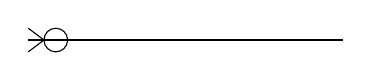
\begin{tikzpicture}
\draw (0,0) -- (4,0);
\draw (0,0.15) -- (0.2,0) -- (0,-0.15);
\draw (0.35,0) circle (0.15);
\end{tikzpicture}
\hspace{0.5cm}
\parbox[t]{11cm}{Zero or More}

\noindent
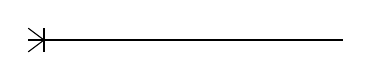
\begin{tikzpicture}
\draw (0,0) -- (4,0);
\draw (0,0.15) -- (0.2,0) -- (0,-0.15);
\draw (0.2,0.15) -- (0.2,-0.15);
\end{tikzpicture}
\hspace{0.5cm}
\parbox[t]{11cm}{One or More}

\noindent
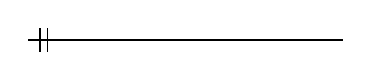
\begin{tikzpicture}
\draw (0,0) -- (4,0);
\draw (0.15,0.15) -- (0.15,-0.15);
\draw (0.25,0.15) -- (0.25,-0.15);
\end{tikzpicture}
\hspace{0.5cm}
\parbox[t]{11cm}{One and only One}

\noindent
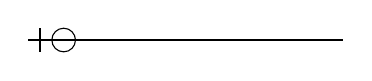
\begin{tikzpicture}
\draw (0,0) -- (4,0);
\draw (0.15,0.15) -- (0.15,-0.15);
\draw (0.45,0) circle (0.15);
\end{tikzpicture}
\hspace{0.5cm}
\parbox[t]{11cm}{Zero or One}

\subsection{Many-to-One}

\noindent
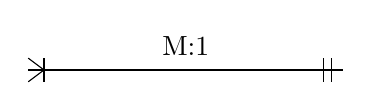
\begin{tikzpicture}
\draw (0,0) -- (4,0);
\draw (0,0.15) -- (0.2,0) -- (0,-0.15);
\draw (0.2,0.15) -- (0.2,-0.15);
\draw (3.75,0.15) -- (3.75,-0.15);
\draw (3.85,0.15) -- (3.85,-0.15);
\node at (2,0.3) {M:1};
\end{tikzpicture}
\hspace{0.5cm}
\parbox[t]{11cm}{a one through many notation on one side of a relationship and a one and only one on the other}

\noindent
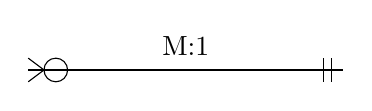
\begin{tikzpicture}
\draw (0,0) -- (4,0);
\draw (0,0.15) -- (0.2,0) -- (0,-0.15);
\draw (0.35,0) circle (0.15);
\draw (3.75,0.15) -- (3.75,-0.15);
\draw (3.85,0.15) -- (3.85,-0.15);
\node at (2,0.3) {M:1};
\end{tikzpicture}
\hspace{0.5cm}
\parbox[t]{11cm}{a zero through many notation on one side of a relationship and a one and only one on the other}

\noindent
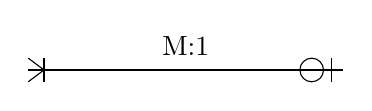
\begin{tikzpicture}
\draw (0,0) -- (4,0);
\draw (0,0.15) -- (0.2,0) -- (0,-0.15);
\draw (0.2,0.15) -- (0.2,-0.15);
\draw (3.6,0) circle (0.15);
\draw (3.85,0.15) -- (3.85,-0.15);
\node at (2,0.3) {M:1};
\end{tikzpicture}
\hspace{0.5cm}
\parbox[t]{11cm}{a one through many notation on one side of a relationship and a zero or one notation on the other}

\noindent
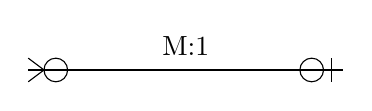
\begin{tikzpicture}
\draw (0,0) -- (4,0);
\draw (0,0.15) -- (0.2,0) -- (0,-0.15);
\draw (0.35,0) circle (0.15);
\draw (3.6,0) circle (0.15);
\draw (3.85,0.15) -- (3.85,-0.15);
\node at (2,0.3) {M:1};
\end{tikzpicture}
\hspace{0.5cm}
\parbox[t]{11cm}{a zero through many notation on one side of a relationship and a zero or one notation on the other}

\subsection{Many-to-Many}

\noindent
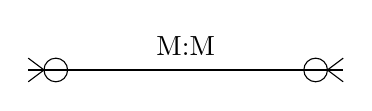
\begin{tikzpicture}
\draw (0,0) -- (4,0);
\draw (0,0.15) -- (0.2,0) -- (0,-0.15);
\draw (0.35,0) circle (0.15);
\draw (3.65,0) circle (0.15);
\draw (4,0.15) -- (3.8,0) -- (4,-0.15);
\node at (2,0.3) {M:M};
\end{tikzpicture}
\hspace{0.5cm}
\parbox[t]{11cm}{a zero through many on both sides of a relationship}

\noindent
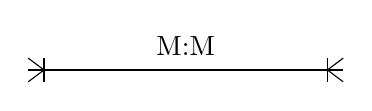
\begin{tikzpicture}
\draw (0,0) -- (4,0);
\draw (0,0.15) -- (0.2,0) -- (0,-0.15);
\draw (0.2,0.15) -- (0.2,-0.15);
\draw (3.8,0.15) -- (3.8,-0.15);
\draw (4,0.15) -- (3.8,0) -- (4,-0.15);
\node at (2,0.3) {M:M};
\end{tikzpicture}
\hspace{0.5cm}
\parbox[t]{11cm}{a one through many on both sides of a relationship}

\noindent
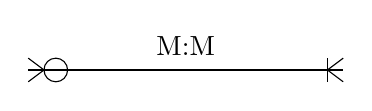
\begin{tikzpicture}
\draw (0,0) -- (4,0);
\draw (0,0.15) -- (0.2,0) -- (0,-0.15);
\draw (0.35,0) circle (0.15);
\draw (3.8,0.15) -- (3.8,-0.15);
\draw (4,0.15) -- (3.8,0) -- (4,-0.15);
\node at (2,0.3) {M:M};
\end{tikzpicture}
\hspace{0.5cm}
\parbox[t]{11cm}{a zero through many on one side and a one through many on the other}

\subsection{One-to-One}

\noindent
\begin{tikzpicture}
\draw (0,0) -- (4,0);
\draw (0.15,0.15) -- (0.15,-0.15);
\draw (0.25,0.15) -- (0.25,-0.15);
\draw (3.6,0) circle (0.15);
\draw (3.85,0.15) -- (3.85,-0.15);
\node at (2,0.3) {1:1};
\end{tikzpicture}
\hspace{0.5cm}
\parbox[t]{11cm}{a one and only one notation on one side of a relationship and a zero or one on the other}

\noindent
\begin{tikzpicture}
\draw (0,0) -- (4,0);
\draw (0.15,0.15) -- (0.15,-0.15);
\draw (0.25,0.15) -- (0.25,-0.15);
\draw (3.75,0.15) -- (3.75,-0.15);
\draw (3.85,0.15) -- (3.85,-0.15);
\node at (2,0.3) {1:1};
\end{tikzpicture}
\hspace{0.5cm}
\parbox[t]{11cm}{a one and only one notation on both sides}